% --------------------------------------------------------------
% This is all preamble stuff that you don't have to worry about.
% Head down to where it says "Start here"
% --------------------------------------------------------------

\documentclass[12pt]{article}

\usepackage[margin=1in]{geometry}
\usepackage{amsmath,amsthm,amssymb}
\usepackage{enumerate}
\usepackage{graphicx}
\usepackage[english]{babel}
\usepackage[utf8x]{inputenc}
\usepackage[T1]{fontenc}
\usepackage{enumitem}
\usepackage{fancyhdr}
\pagestyle{fancy}
\usepackage[table,xcdraw]{xcolor}

\newcommand{\N}{\mathbb{N}}
\newcommand{\Z}{\mathbb{Z}}
\newcommand{\R}{\mathbb{R}}
\newcommand{\Q}{\mathbb{Q}}
\newcommand{\C}{\mathbb{C}}

\newenvironment{theorem}[2][Theorem]{\begin{trivlist}
\item[\hskip \labelsep {\bfseries #1}\hskip \labelsep {\bfseries #2.}]}{\end{trivlist}}
\newenvironment{lemma}[2][Lemma]{\begin{trivlist}
\item[\hskip \labelsep {\bfseries #1}\hskip \labelsep {\bfseries #2.}]}{\end{trivlist}}
\newenvironment{exercise}[2][Exercise]{\begin{trivlist}
\item[\hskip \labelsep {\bfseries #1}\hskip \labelsep {\bfseries #2.}]}{\end{trivlist}}
\newenvironment{problem}[2][Problem]{\begin{trivlist}
\item[\hskip \labelsep {\bfseries #1}\hskip \labelsep {\bfseries #2.}]}{\end{trivlist}}
\newenvironment{question}[2][Question]{\begin{trivlist}
\item[\hskip \labelsep {\bfseries #1}\hskip \labelsep {\bfseries #2.}]}{\end{trivlist}}
\newenvironment{corollary}[2][Corollary]{\begin{trivlist}
\item[\hskip \labelsep {\bfseries #1}\hskip \labelsep {\bfseries #2.}]}{\end{trivlist}}

\lhead{Report 1, October 17, 2022}
\rhead{Nicholas Tee}

\begin{document}

\subsection*{Benchmark 1: spec00-bzip2}
These are the cache values from the \textbf{bzip2} benchmark without any changes.\\
\textbf{Instruction Count:} 362,993,028\\
\textbf{Cycle Count:} 417,769,347\\
\textbf{Sampler:} TASS\\
\begin{table}[!h]
\centering
\begin{tabular}{|l|l|l|l|l|l|l|l|}
\hline
\rowcolor[HTML]{C0C0C0} 
Cache & Average Memory Latency & MemAccesses & MissRate1 & MissRate2 & RD & WR & BUS \\ \hline
\cellcolor[HTML]{EFEFEF}IL1 & 2.0 & 238,638,066 & 0\% & 0\% & 100\% & 0\% & 0\% \\ \hline
\cellcolor[HTML]{EFEFEF}DL1 & 9.1 & 114,584,807 & 2.7\% & 4.5\% & 96.9\% & 95.7\% & 0\% \\ \hline
\cellcolor[HTML]{EFEFEF}L2 & 63.6 & 3,124,247 & 66.8\% & 66.8\% & 33.2\% & 0\% & 0\% \\ \hline
\cellcolor[HTML]{EFEFEF}Memory & 60 & 1,936,828 & 0\% & 0\% & 100\% & 100\% & 0\% \\ \hline
\end{tabular}
\end{table}\\
For the first parameter change, I wanted to see what would happen if I increase the associativity of the \textbf{IL1 cache from 4 to 8}. I was expecting an increase in the miss rate, hoping that there would be a slight increase in the number of capacity misses. Here are the results.
\begin{table}[!h]
\centering
\begin{tabular}{|l|l|l|l|l|l|l|l|}
\hline
\rowcolor[HTML]{C0C0C0} 
Cache & Average Memory Latency & MemAccesses & MissRate1 & MissRate2 & RD & WR & BUS \\ \hline
IL1 & 2.0 & 238,638,068 & 0\% & 0\% & 100\% & 0\% & 0\% \\ \hline
DL1 & 9.0 & 114,584,600 & 2.7\% & 4.5\% & 96.9\% & 95.7\% & 0\% \\ \hline
L2 & 63.6 & 3,093,261 & 66.6\% & 66.6\% & 33.4\% & 0\% & 0\% \\ \hline
Memory & 60 & 1,916,468 & 0\% & 0\% & 100\% & 100\% & 0\% \\ \hline
\end{tabular}
\end{table}\\
Most of the benchmark results did not change except for a slight decrease in the hit rate of the \textbf{L2} cache. I'm not quite sure why this happened, my assumption is that some of the data had been pushed down to a lower level which resulted in more hits. Specifically, an increase in 0.2\% for the hit rate of read instructions.\\

The next change was a decrease in the block size of the \textbf{DL1 cache from 32 to 8}. I expected an increase in the miss rate if I were to decrease the spacial locality of that level. With an increased miss rate with the L1 cache, I was also expecting an increase in the number of memory accesses for L2. Here are the results.
\begin{table}[!h]
\centering
\begin{tabular}{|l|l|l|l|l|l|l|l|}
\hline
\rowcolor[HTML]{C0C0C0} 
Cache & Average Memory Latency & MemAccesses & MissRate1 & MissRate2 & RD & WR & BUS \\ \hline
IL1 & 2.0 & 238,638,068 & 0\% & 0\% & 100\% & 0\% & 0\% \\ \hline
DL1 & 9.2 & 114,584,600 & 4.9\% & 7.4\% & 94.7\% & 93.1\% & 0\% \\ \hline
L2 & 63.6 & 5,620,958 & 35.2\% & 38.9\% & 63.4\% & 0\% & 0\% \\ \hline
Memory & 60 & 1,762,288 & 0\% & 0\% & 100\% & 100\% & 0\% \\ \hline
\end{tabular}
\end{table}
As expected, there was an increase in miss rate for DL1 and in the number of memory accesses for L2. Although for a decrease in bloack size from 32 to 8, I was expecting a much larger increase in miss rate. I also did not expect the miss rate of the L2 cache to decrease as much as it did. I assume this is due to a lot of data having to be pushed down to L2 instead of being stored in L1, which would then lead to an increase in its hit rate.
\newpage
\subsection*{Benchmark 2: spec00-crafty}
\textbf{Instruction Count:} 362,993,023\\
\textbf{Cycle Count:} 406,031,896\\
\textbf{Sampler:} TASS\\
\begin{table}[!h]
\centering
\begin{tabular}{|l|l|l|l|l|l|l|l|}
\hline
\rowcolor[HTML]{C0C0C0} 
Cache & Average Memory Latency & MemAccesses & MissRate1 & MissRate2 & RD & WR & BUS \\ \hline
IL1 & 2.3 & 235,407,812 & 0.2\% & 0.4\% & 99.8\% & 0\% & 0\% \\ \hline
DL1 & 7.1 & 116,117,768 & 0.6\% & 0.7\% & 99.1\% & 99.9\% & 0\% \\ \hline
L2 & 77.1 & 1,075,601 & 97.0\% & 97.0\% & 3.0\% & 0\% & 0\% \\ \hline
Memory & 60 & 1,023,978 & 0\% & 0\% & 100\% & 100\% & 0\% \\ \hline
\end{tabular}
\end{table}\\
First change was to \textbf{increase block size of DL1 from 32 to 64}. Based on the previous benchmark, I was expecting a small increase or decrease of miss rate, since I would be increasing spatial locality, but decreasing temporal locality. Without knowing exactly what the benchmarks are performing, it would be difficult to make an educated guess of the effects.\\
\begin{table}[!h]
\centering
\begin{tabular}{|l|l|l|l|l|l|l|l|}
\hline
\rowcolor[HTML]{C0C0C0} 
Cache & Average Memory Latency & MemAccesses & MissRate1 & MissRate2 & RD & WR & BUS \\ \hline
IL1 & 2.3 & 235,407,809 & 0.2\% & 0.4\% & 99.8\% & 0\% & 0\% \\ \hline
DL1 & 7.1 & 116,117,175 & 0.7\% & 0.9\% & 98.9\% & 99.8\% & 0\% \\ \hline
L2 & 55.3 & 1,235,659 & 59.0\% & 59.9\% & 40.1\% & 0\% & 0\% \\ \hline
Memory & 60 & 727,730 & 0\% & 0\% & 100\% & 100\% & 0\% \\ \hline
\end{tabular}
\end{table}
There would be an minuscule increase in the miss rate of DL1, but a quite significant decrease in the miss rate of the L2 cache. Similar to the previous benchmark, this was probably due to the L1 cache not being able to hold as much data as before. There was also a decrease in the number of memory accesses from main memory.\\

The next change was to \textbf{decrease associativity of DL1 from 4 to direct-mapped}. I was attempting to make a more significant change to the hit rate of DL1 since all the previous changes have been small. The results are as follows
\begin{table}[!h]
\centering
\begin{tabular}{|l|l|l|l|l|l|l|l|}
\hline
\rowcolor[HTML]{C0C0C0} 
Cache & Average Memory Latency & MemAccesses & MissRate1 & MissRate2 & RD & WR & BUS \\ \hline
IL1 & 2.3 & 235,407,809 & 0.2\% & 0.4\% & 99.8\% & 0\% & 0\% \\ \hline
DL1 & 9.8 & 116,117,045 & 3.7\% & 4.6\% & 95.1\% & 97.6\% & 0\% \\ \hline
L2 & 71.9 & 4,704,187 & 92.6\% & 92.6\% & 7.4\% & 0\% & 0\% \\ \hline
Memory & 60 & 3,957,805 & 0\% & 0\% & 100\% & 100\% & 0\% \\ \hline
\end{tabular}
\end{table}\\
As hoped, the change created a much more significant change. By changing the associativity of the L1 cache from 4 to being direct-mapped, there was a significant increase of misses overall. A 3\% increase in primary misses for L1 is the largest change I have observed so far. Furthermore, although there was technically a slight decrease in miss rate for L2, the number of memory accesses increased significantly, which results in more misses in general.
\newpage
\subsection*{Benchmark 3: spec00-gcc}
\textbf{Instruction Count:} 362,993,023\\
\textbf{Cycle Count:} 822,813,193\\
\textbf{Sampler:} TASS\\
For these tests I wanted to try and affect the sim time instead of playing with the cache parameters. Here are the base values
\begin{table}[!h]
\begin{tabular}{|l|l|l|l|l|}
\hline
\rowcolor[HTML]{C0C0C0} 
                             & Rabbit & Warmup & Detail & Timing \\ \hline
\cellcolor[HTML]{C0C0C0}KIPS & 97816  & N/A    & 517248 & 1308   \\ \hline
\cellcolor[HTML]{C0C0C0}Time & 11.6\% & 0\%    & 1.8\%  & 86.6\% \\ \hline
\cellcolor[HTML]{C0C0C0}Inst & 51.8\% & 0\%    & 43\%   & 5.2\%  \\ \hline
\end{tabular}
\end{table}\\
\textbf{Simulation Time:} 347.499 seconds\\

For the first change, I reduced the L3(I assume this is main memory) \textbf{size from 2GB to 1GB}. I was expecting a large increase in the simulation time, and perhaps an increase in miss rate for memory. Here are the results

\begin{table}[!h]
\begin{tabular}{|l|l|l|l|l|}
\hline
\rowcolor[HTML]{C0C0C0} 
                             & Rabbit & Warmup & Detail & Timing \\ \hline
\cellcolor[HTML]{C0C0C0}KIPS & 102904 & N/A    & 248056 & 11288  \\ \hline
\cellcolor[HTML]{C0C0C0}Time & 5.7\%  & 0\%    & 2\%    & 92.4\% \\ \hline
\cellcolor[HTML]{C0C0C0}Inst & 51.8\% & 0\%    & 43\%   & 5.2\%  \\ \hline
\end{tabular}
\end{table}
\textbf{Simulation Time:} 648.099 seconds\\
As expected, the total simulation time doubled entirely from reducing the size of memory. Sadly, there were no changes to the miss rates of any of the caches, which is why none of the values are currently displayed. However, I was confused as to why the IPC did not change, as I had initially thought that the reducing in memory capacity would have at least a minor effect.\\

The next change was to the \textbf{instruction queue size from 24 to 12}. I am expecting changes similar to that of the previous benchmark test, here are the results.

\begin{table}[!h]
\begin{tabular}{|l|l|l|l|l|}
\hline
\rowcolor[HTML]{C0C0C0} 
                             & Rabbit & Warmup & Detail & Timing \\ \hline
\cellcolor[HTML]{C0C0C0}KIPS & 101110 & N/A    & 244754 & 11199  \\ \hline
\cellcolor[HTML]{C0C0C0}Time & 5.7\%  & 0\%    & 2\%    & 92.4\% \\ \hline
\cellcolor[HTML]{C0C0C0}Inst & 51.8\% & 0\%    & 43\%   & 5.2\%  \\ \hline
\end{tabular}
\end{table}
\textbf{Simulation Time:} 653.169 seconds\\
Similar to the previous test, I was expecting more changes to the CPU's general performance, but the only thing that changed was the massive increase in simulation time as well. This effect makes sense as the CPU can only look at half the instructions at a time.

\newpage
\subsection*{Benchmark 4: spec00-gzip}
\textbf{Instruction Count:} 362,993,053\\
\textbf{Cycle Count:} 352,727,393\\
\textbf{Sampler:} TASS\\
\begin{table}[!h]
\centering
\begin{tabular}{|l|l|l|l|l|l|l|l|}
\hline
\rowcolor[HTML]{C0C0C0} 
Cache & Average Memory Latency & MemAccesses & MissRate1 & MissRate2 & RD & WR & BUS \\ \hline
IL1 & 2 & 237,010,544 & 0\% & 0\$ & 100\% & 0\% & 0\% \\ \hline
DL1 & 11.4 & 101,478,498 & 2.5\% & 6.6\% & 97.8\% & 90.0\% & 0\% \\ \hline
L2 & 67.6 & 2,504,678 & 33.9\% & 33.9\% & 66.1\% & 0\% & 0\% \\ \hline
Memory & 60 & 1,371,981 & 0\% & 0\% & 100\% & 100\% & 0\% \\ \hline
\end{tabular}
\end{table}\\
The first parameter change was to \textbf{completely remove the IL1} cache. I wanted to see the effect it would have by removing a whole level of the cache. I expect to have an increase in memory accesses for DL1 and perhaps a change in the miss rate for all the lower level caches. Here were the results

\begin{table}[!h]
\centering
\begin{tabular}{|l|l|l|l|l|l|l|l|}
\hline
\rowcolor[HTML]{C0C0C0} 
Cache & Average Memory Latency & MemAccesses & MissRate1 & MissRate2 & RD & WR & BUS \\ \hline
IL1 & - & - & - & - & - & - & - \\ \hline
DL1 & 11.4 & 101,478,498 & 2.5\% & 6.6\% & 97.8\% & 90.0\% & 0\% \\ \hline
L2 & 67.6 & 2,504,025 & 33.9\% & 33.9\% & 66.1\% & 0\% & 0\% \\ \hline
Memory & 60 & 1,371,085 & 0\% & 0\% & 100\% & 100\% & 0\% \\ \hline
\end{tabular}
\end{table}
For some reason nothing had changed except for the fact the IL1 cache was missing from the report, I was sure that I did it correctly, so I am unsure as to why none of the values had changed. I expected the number of memory accesses to change for DL1 but it had stayed the exact same.\\

This time I wanted to \textbf{remove DL1} instead and see if there would be any change. Because of the previous benchmark test not having any affect, I expect the same from this one. Here are the results
\begin{table}[!h]
\centering
\begin{tabular}{|l|l|l|l|l|l|l|l|}
\hline
\rowcolor[HTML]{C0C0C0} 
Cache & Average Memory Latency & MemAccesses & MissRate1 & MissRate2 & RD & WR & BUS \\ \hline
IL1 & 2.0 & 237,010,637 & 0\% & 0\% & 100\% & 0\% & 0\% \\ \hline
DL1 & - & - & - & - & - & - & - \\ \hline
L2 & 67.6 & 425 & 99.8\% & 99.8\% & 0\% & 0\% & 0\% \\ \hline
Memory & 60 & 425 & 0\% & 0\% & 99.9\% & 100\% & 0\% \\ \hline
\end{tabular}
\end{table}\\
Due to the removal of the DL1 cache, there was a significant decrease in memory accesses from L2 and main memory, which basically no hits. I am still unsure as to why this is the case, as I would have though there would be an increase in memory accesses with the lower levels. I might have changed the parameters incorrectly in my bash script.
\newpage
\section*{Appendix}
\textbf{bzip2: base}
\begin{figure}[h!]
	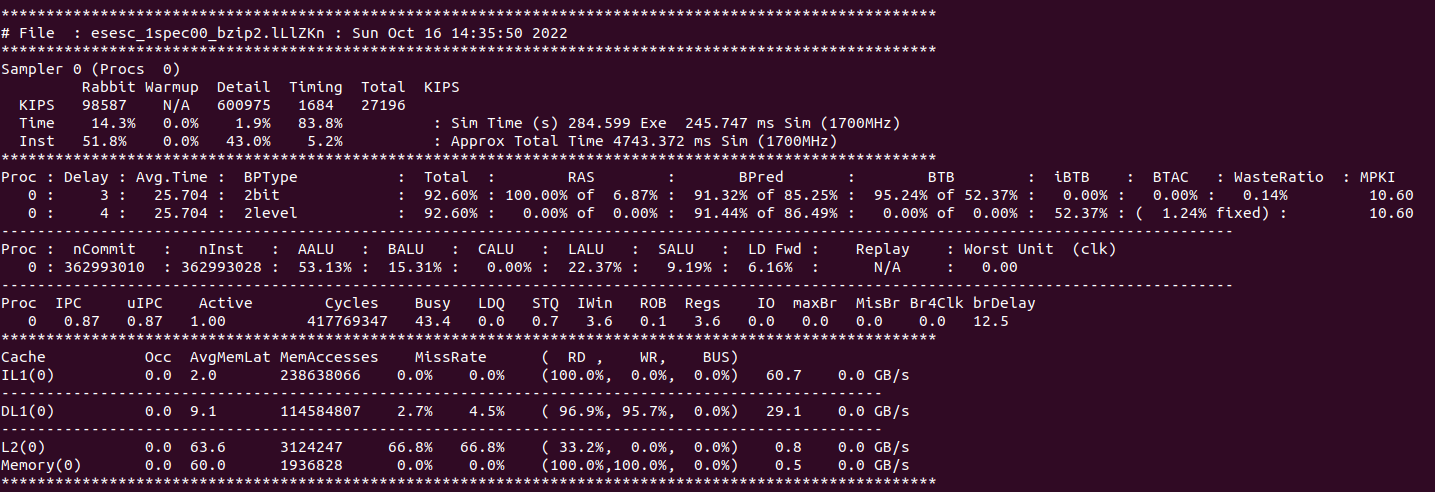
\includegraphics[scale=0.4]{img/bzip1.png}
\end{figure}

\textbf{bzip2: IL1 associativity from 4 to 8}
\begin{figure}[h!]
	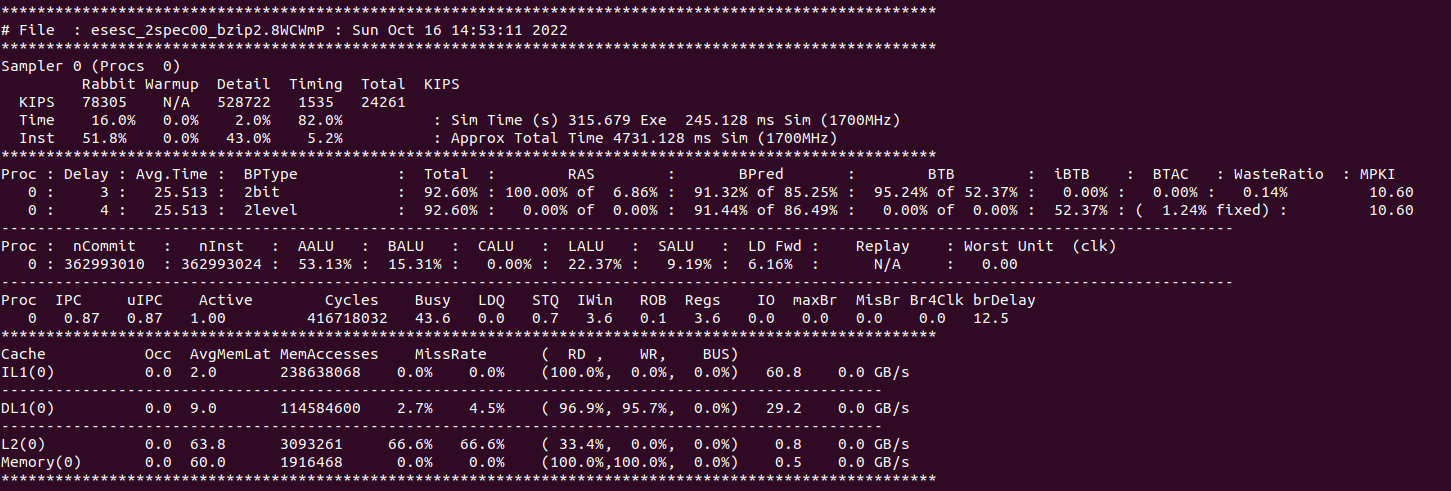
\includegraphics[scale=0.4]{img/bzip2.png}
\end{figure}

\textbf{bzip2: DL1 block size from 32 to 8}
\begin{figure}[h!]
	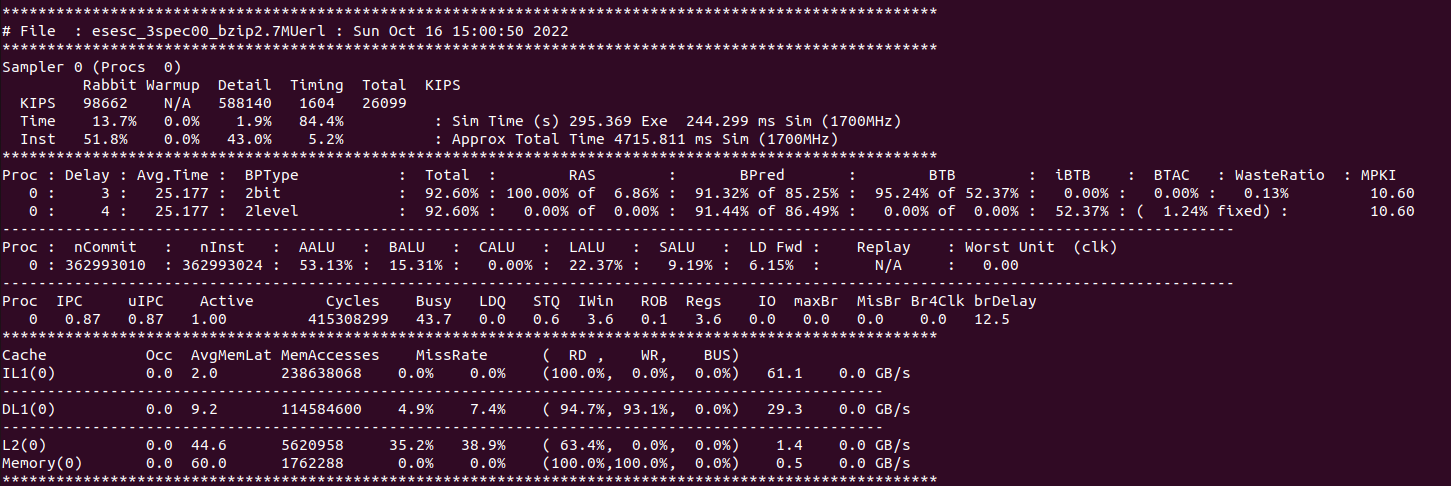
\includegraphics[scale=0.4]{img/bzip3.png}
\end{figure}
\newpage

\textbf{crafty: base}
\begin{figure}[h!]
	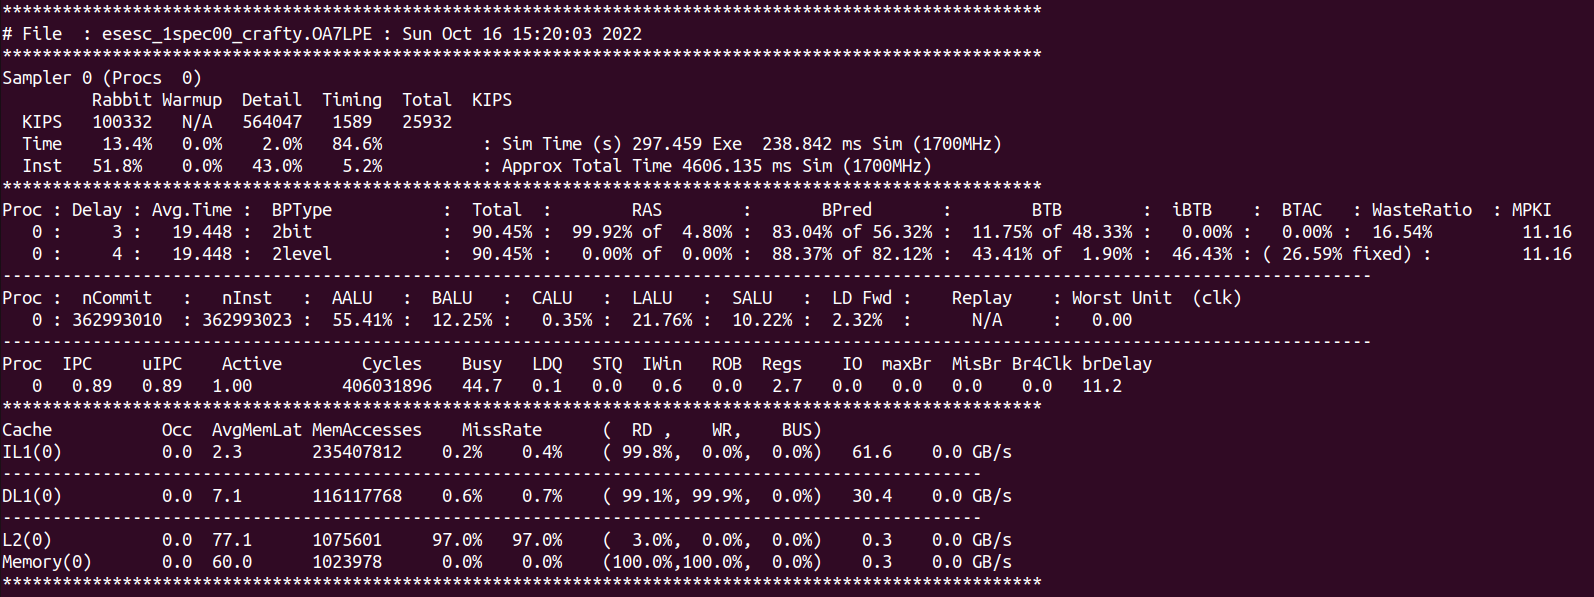
\includegraphics[scale=0.3]{img/crafty1.png}
\end{figure}

\textbf{crafty: DL1 block size from 32 to 64}
\begin{figure}[h!]
	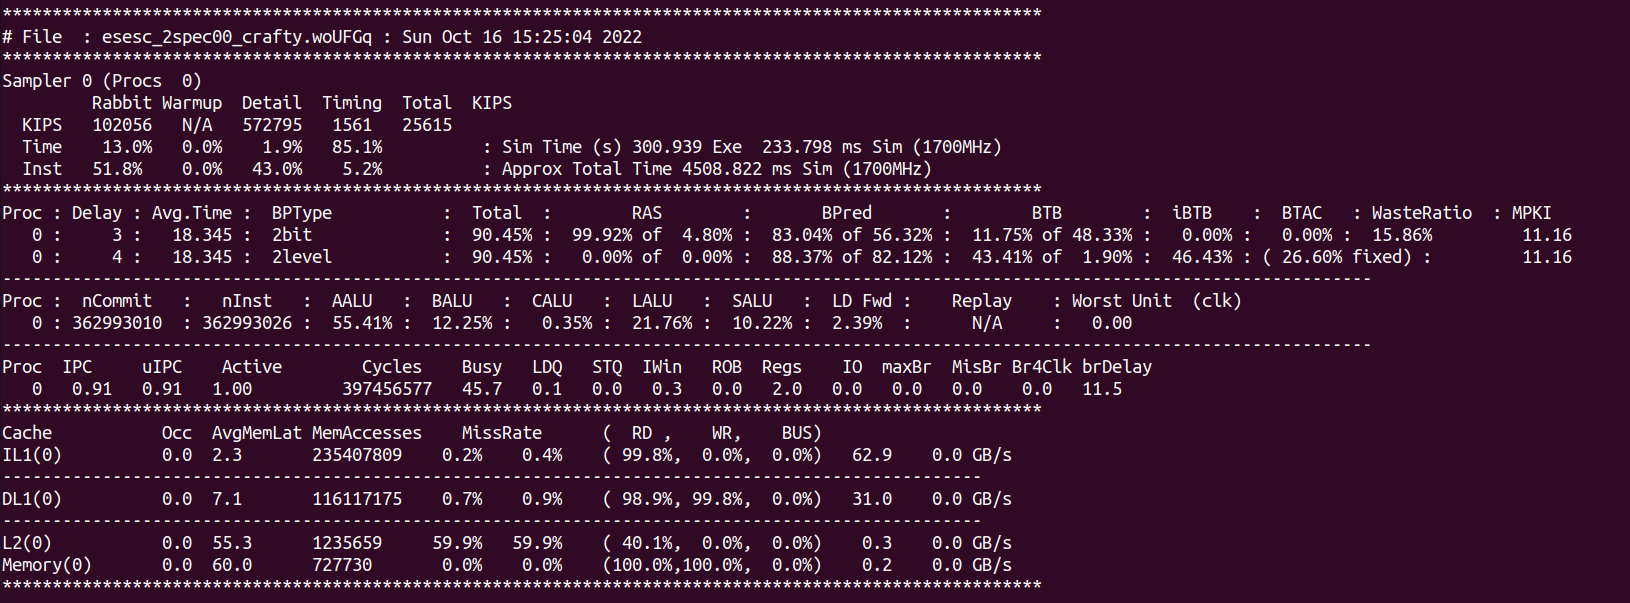
\includegraphics[scale=0.3]{img/crafty2.png}
\end{figure}

\textbf{crafty: DL1 associativity from 4 to 1}
\begin{figure}[h!]
	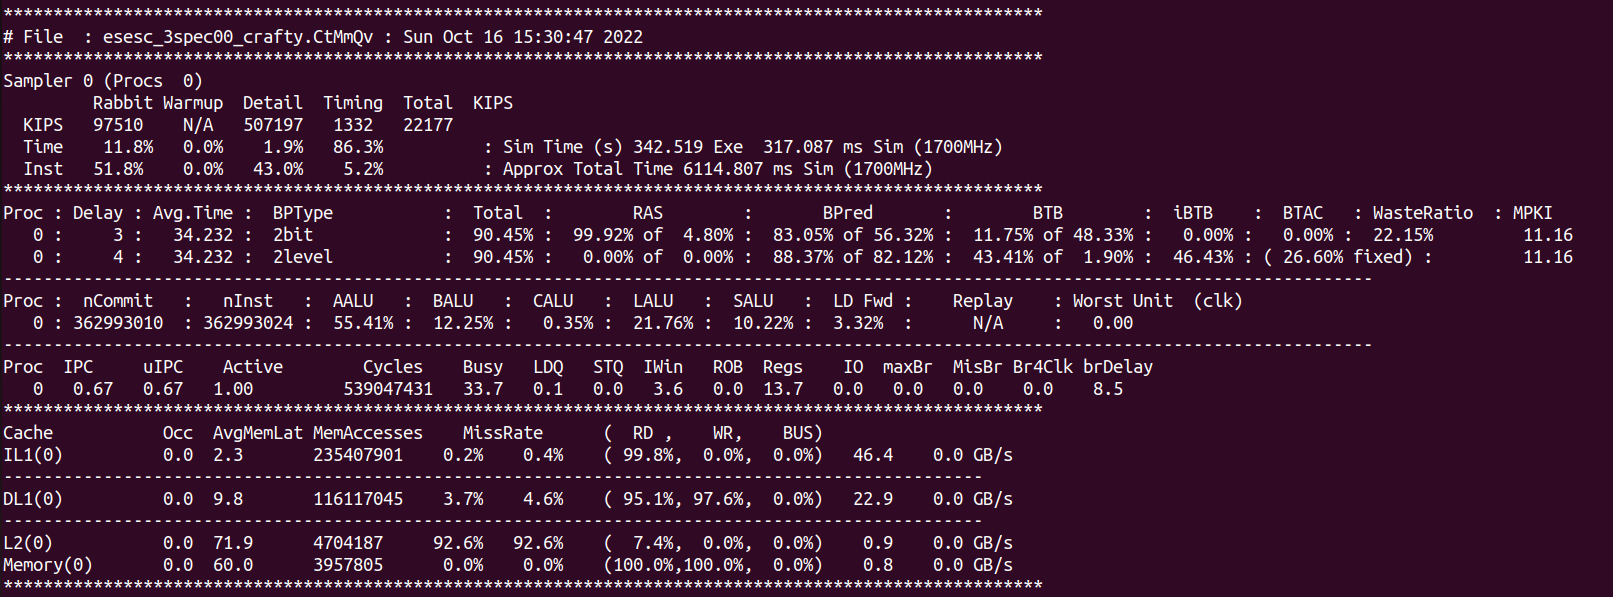
\includegraphics[scale=0.3]{img/crafty3.png}
\end{figure}
\newpage

\textbf{gcc: base}
\begin{figure}[h!]
	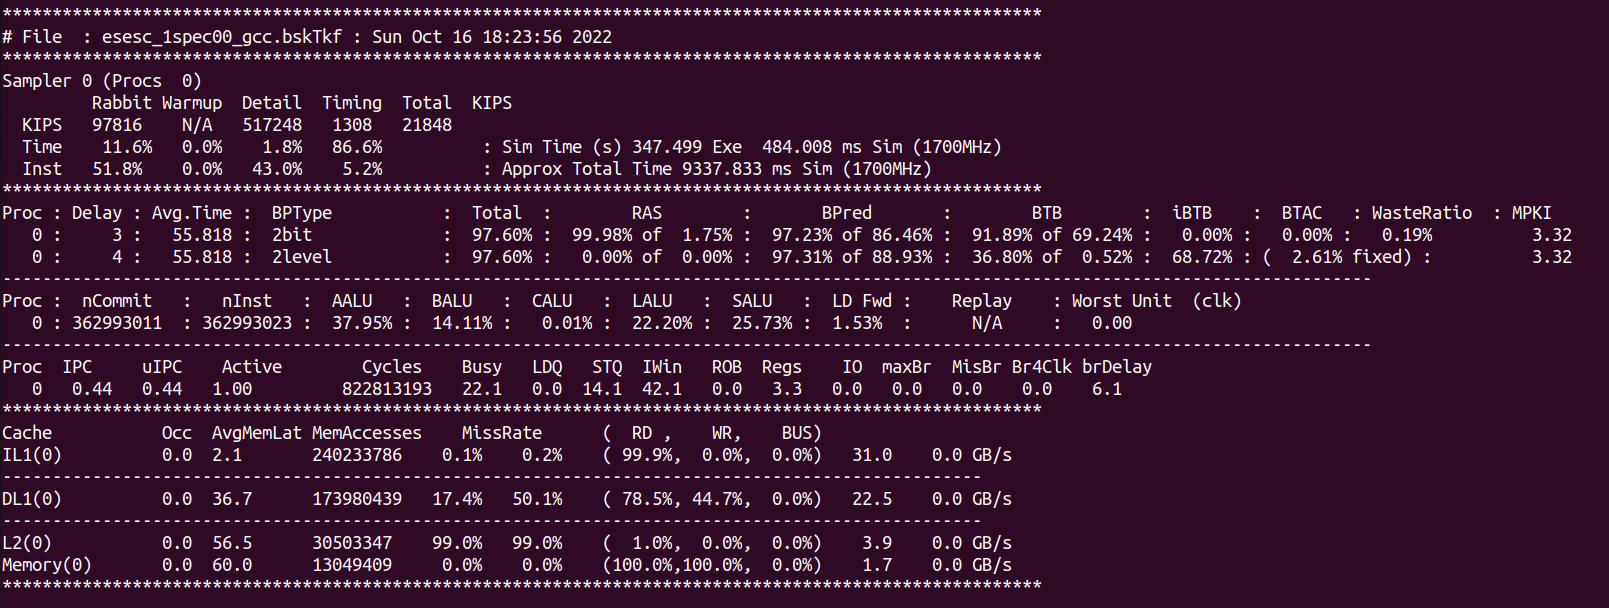
\includegraphics[scale=0.3]{img/gcc1.png}
\end{figure}

\textbf{gcc: L3 size from 2GB to 1GB}
\begin{figure}[h!]
	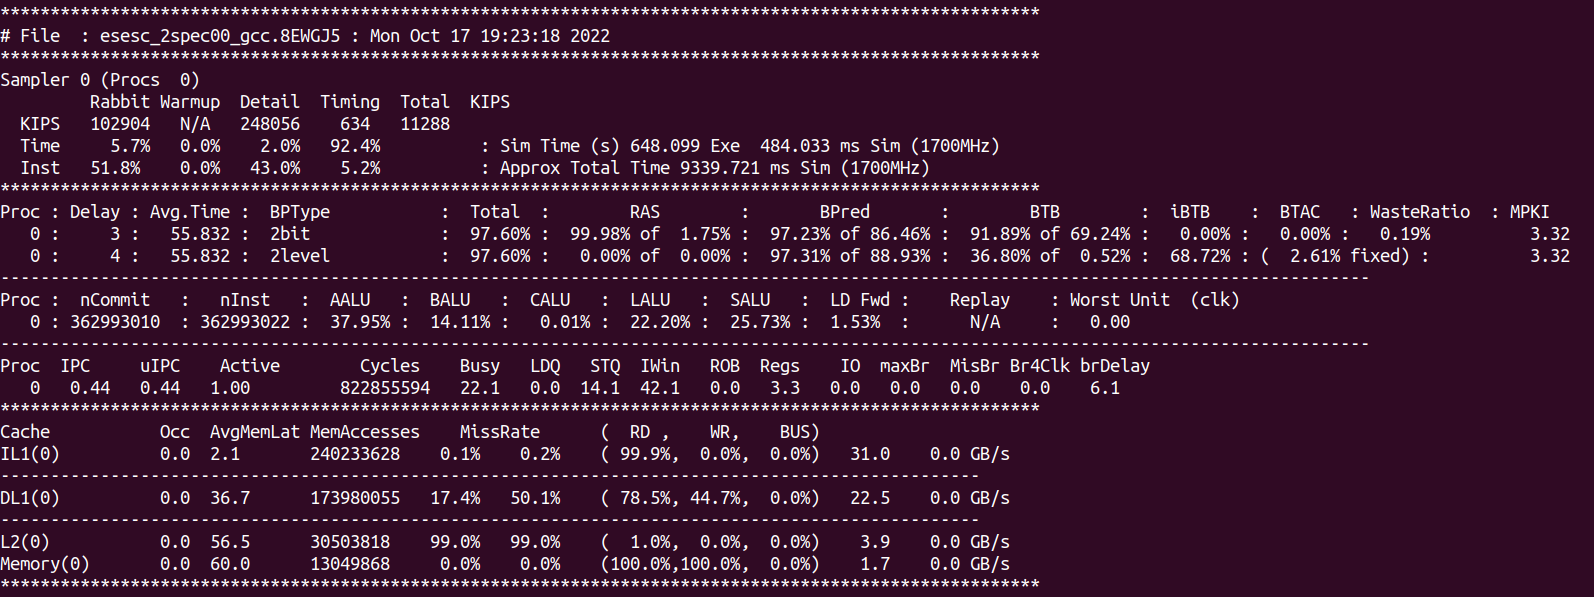
\includegraphics[scale=0.3]{img/gcc2.png}
\end{figure}

\textbf{gcc: Instruction queue from 24 to 12}
\begin{figure}[h!]
	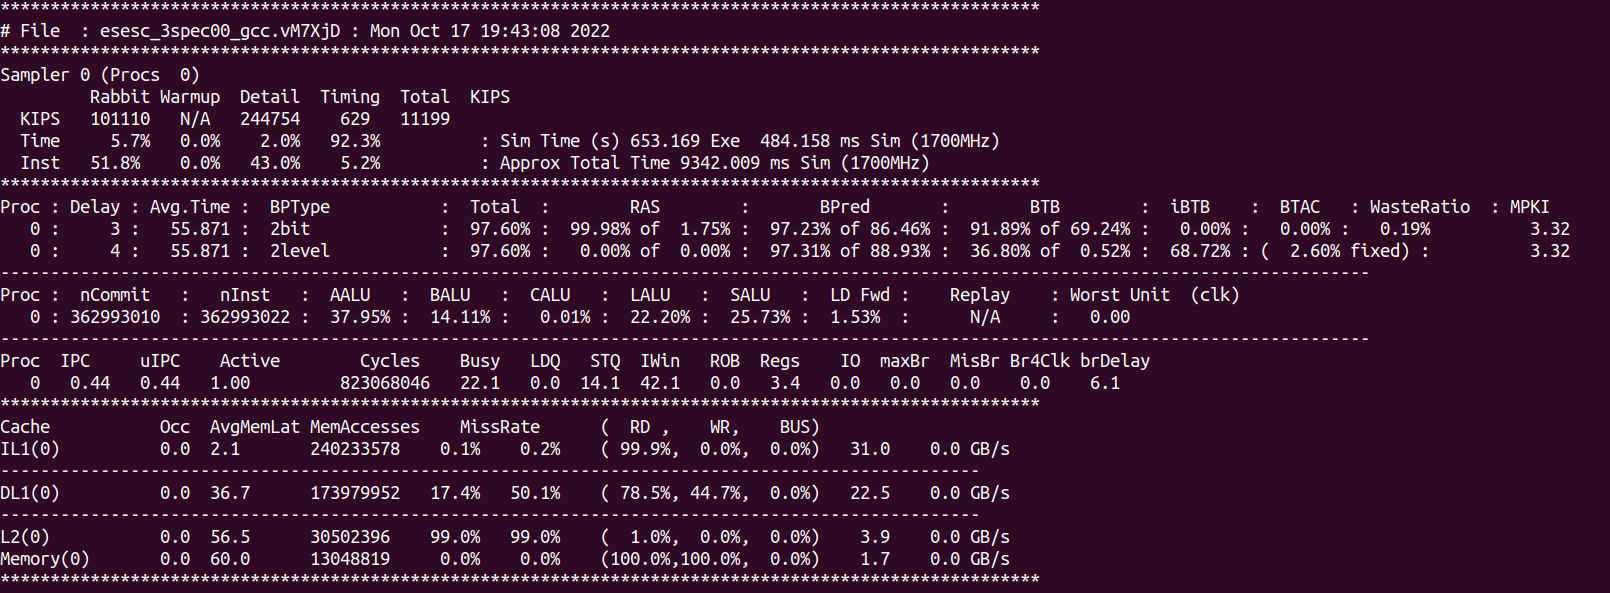
\includegraphics[scale=0.3]{img/gcc3.png}
\end{figure}

\newpage

\textbf{gzip: base}
\begin{figure}[h!]
	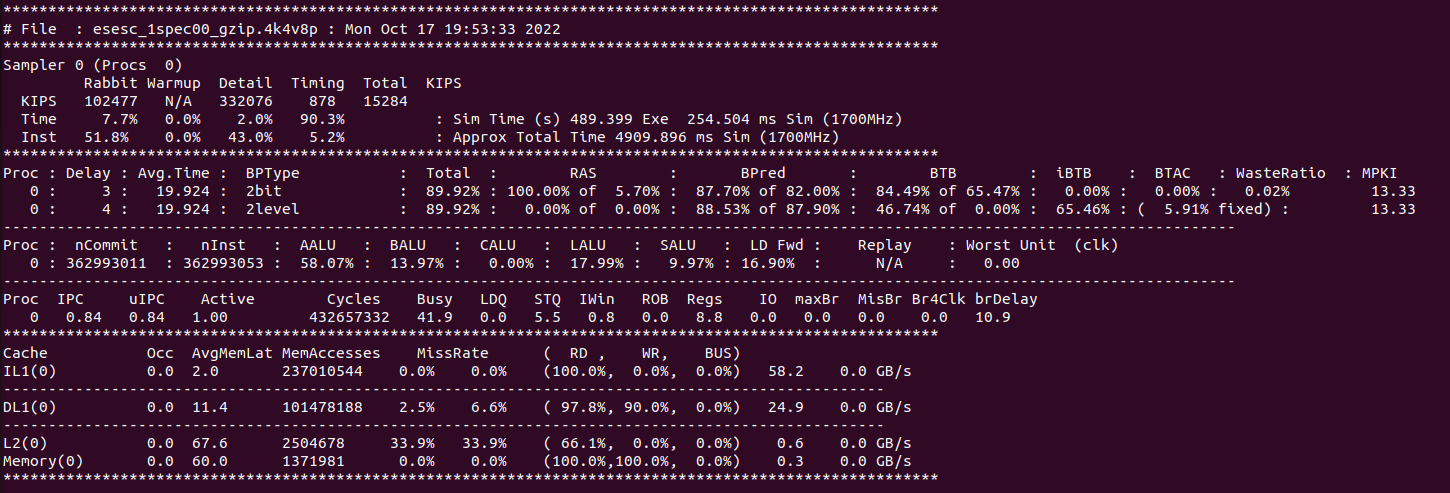
\includegraphics[scale=0.3]{img/gzip1.png}
\end{figure}

\textbf{gzip: IL1 removed}
\begin{figure}[h!]
	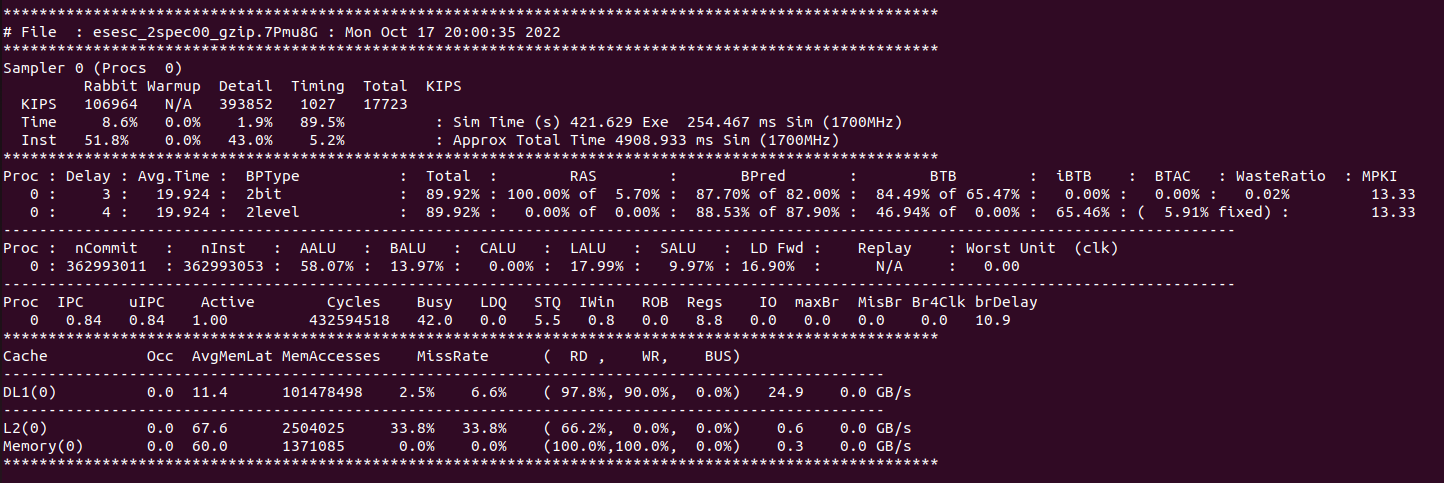
\includegraphics[scale=0.3]{img/gzip2.png}
\end{figure}

\textbf{gzip: DL1 removed}
\begin{figure}[h!]
	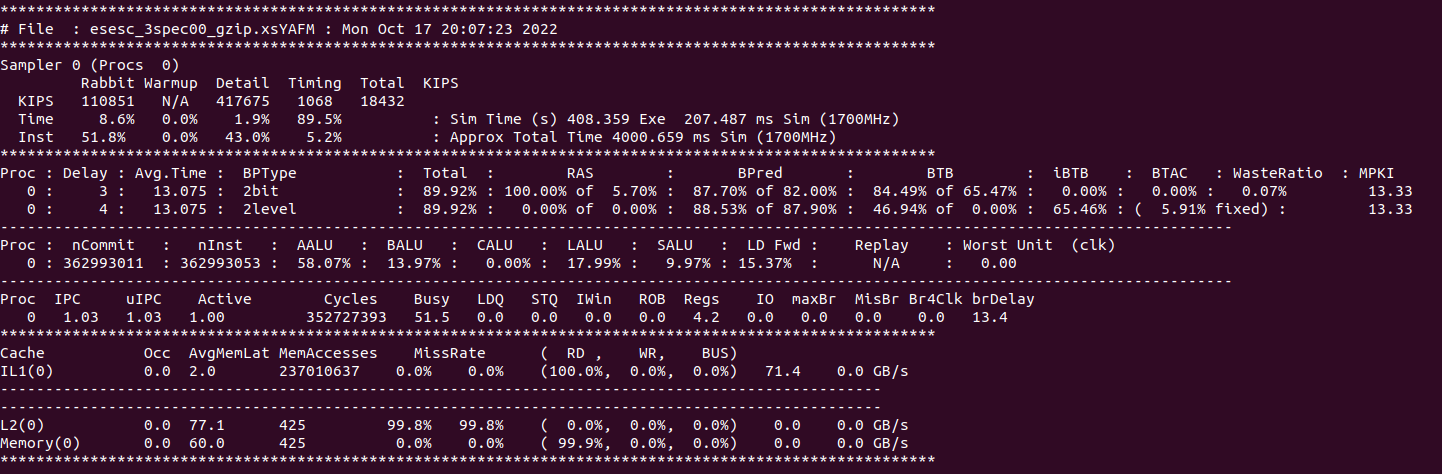
\includegraphics[scale=0.3]{img/gzip3.png}
\end{figure}

\end{document}